%%%%%%%%%%%%%%%%%%%%%%%%
%
% $Autor: Hemanth Jadiswami Prabhakaran $
% $Datum: 2026-09-12 $
% $Pfad: GitHub/MBIDA_Thesis/report/Contents/General/en/08ApplicationDeployment.tex $
% $Version: 1 $
%
% $Project: MBIDA Thesis $
%
%%%%%%%%%%%%%%%%%%%%%%%%

\chapter{Application Deployment}
\label{chap:appDeployment}

This chapter covers the deployed Streamlit dashboard itself: the Parquet data contract between the pipeline and the app (Section~\ref{sec:dataContracts}), the cascading dropdown controls used to navigate the hierarchy (Section~\ref{sec:cascadingDropdowns}), the design of the forecast chart (Section~\ref{sec:chartDesign}), how the app senses the browser's colour theme (Section~\ref{sec:themeSensing}), and how the app is deployed and kept in step with the pipeline's output (Sections~\ref{sec:streamlitDeployment} and~\ref{sec:deploymentFlow}). The pipeline that produces the data read here was implemented in Chapter~\ref{chap:appDevelopment}; \texttt{config.py}, the single source of truth shared between the notebooks and the app, was introduced in Chapter~\ref{chap:devToDeployment}.

\section{Data Contracts}
\label{sec:dataContracts}

The dashboard never re-runs the pipeline itself -- Streamlit Community Cloud only ever executes \texttt{app/streamlit\_app.py} -- so the entire interface between the pipeline and the app is file-based. \texttt{02\_pipeline.ipynb}'s final step exports four Parquet files into \texttt{Code/artifacts/dashboard\_data/}, and the app's \texttt{load\_data()} function reads all four back in on startup:

\begin{itemize}
	\item \texttt{hierarchy.parquet} -- the distinct state/store/category/department/item combinations, with duplicates dropped. This is the lookup table the cascading dropdowns filter against (Section~\ref{sec:cascadingDropdowns}); it carries no dates or sales figures.
	\item \texttt{actuals.parquet} -- the full actual sales history for every hierarchy node, keyed by the series identifier, the date, the sales value, and the train/test/live label produced during data preparation.
	\item \texttt{pred\_with\_gt.parquet} -- the base model forecasts, already restricted to the forecast horizon rather than carrying the full training history.
	\item \texttt{rec\_with\_gt.parquet} -- the reconciled forecasts for the same horizon, with ground truth already attached.
\end{itemize}

Restricting the two forecast files to the horizon, rather than shipping the training-period fitted values as well, keeps the files small enough to commit to the repository alongside the code, in contrast to the gitignored raw data cache. The app wraps \texttt{load\_data()} in \texttt{@st.cache\_data}, so the four files are read once per session rather than on every dropdown interaction.

\section{Cascading Dropdown Interactivity}
\label{sec:cascadingDropdowns}

The sidebar exposes one dropdown per hierarchy level -- State, Store, Category, Department, Item -- each populated from \texttt{hierarchy.parquet} and filtered by every selection made above it: choosing a state restricts the store options to that state's stores, choosing a store restricts the category options to categories sold in that store, and so on down to Item. Every dropdown carries an explicit \texttt{"(All)"} option, and leaving a level on \texttt{"(All)"} stops all levels below it from narrowing further.

These selections are combined into the hierarchy node's identifier by walking State through Item and stopping at the first level left on \texttt{"(All)"}, which mirrors how the pipeline's aggregation spec names its own nodes (\texttt{Total}, \texttt{Total/CA}, \texttt{Total/CA/CA\_1}, and so on down to the bottom level) -- the dropdown ordering is not an independent interface decision, it is the same six-level Total/State/Store/Category/Department/Item structure defined in Section~\ref{sec:hierarchyConstruction}. Leaving every dropdown on \texttt{"(All)"} therefore resolves to \texttt{Total} itself, the grand total series. Because Streamlit's \texttt{selectbox} widgets are searchable by default, a user can also jump straight to a specific store or item by typing rather than scrolling. Alongside the hierarchy controls, a radio button selects the base model and a multiselect chooses one or more reconciliation methods to plot at once; both draw their option lists from \texttt{config.py} so they can never drift out of sync with what the pipeline actually produced. Figure~\ref{fig:dashboardSidebar} shows the sidebar mid-drill-down, with the higher levels resolved to a specific state and store and the remaining levels still open.

\begin{figure}[H]
	\centering
	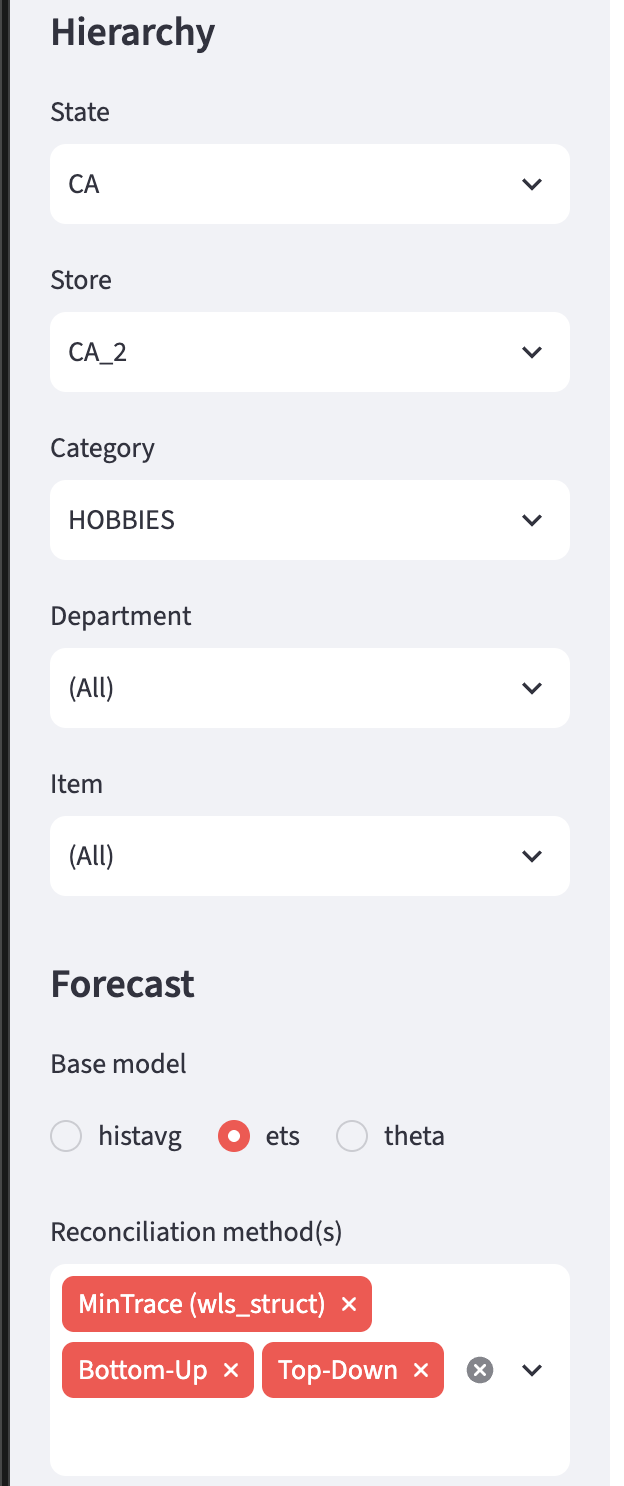
\includegraphics[width=0.6\linewidth]{Images/08ApplicationDeployment/dashboardSidebarControls}
	\caption{The sidebar's cascading dropdown controls, partway through drilling down the hierarchy.}\label{fig:dashboardSidebar}
\end{figure}

\section{Chart Design}
\label{sec:chartDesign}

The forecast chart is built with Plotly and always shows three kinds of trace for the currently selected hierarchy node: the actual sales history, the chosen base forecast, and the chosen reconciled forecast(s). The actual line is drawn only over the train and test periods; the live window is excluded from it entirely, since live-period rows have no real ground truth to plot as if they were observed sales (Section~\ref{sec:timeWindows}). The base forecast is drawn as a dotted line and the reconciled forecast(s) as solid lines, so that even with several reconciliation methods selected at once the base model remains visually distinct from all of them.

Train, test, and live regions are shaded across the full width of the chart using Plotly's \texttt{add\_vrect}, each with its own fill colour and an annotation label, so the three phases are visible at a glance without needing to read axis dates closely -- the same three windows laid out schematically in Figure~\ref{fig:timeWindows}, rendered here interactively for whichever specific series and horizon the user has selected. The chart's background is left fully transparent and its colour palette -- line colour, grid colour, font colour, and shading opacity -- is chosen at render time depending on whether the surrounding app is in light or dark mode (Section~\ref{sec:themeSensing}), so the chart never clashes with the rest of the page. The legend is placed horizontally above the plot area rather than beside it, keeping the full chart width available for the time series itself. Figure~\ref{fig:dashboardChart} shows the resulting chart for the same hierarchy node in both palettes: the shaded train/test/live regions and the dotted base-forecast line are visible in either mode, with only the colour choices differing between them.

\begin{figure}[H]
	\centering
	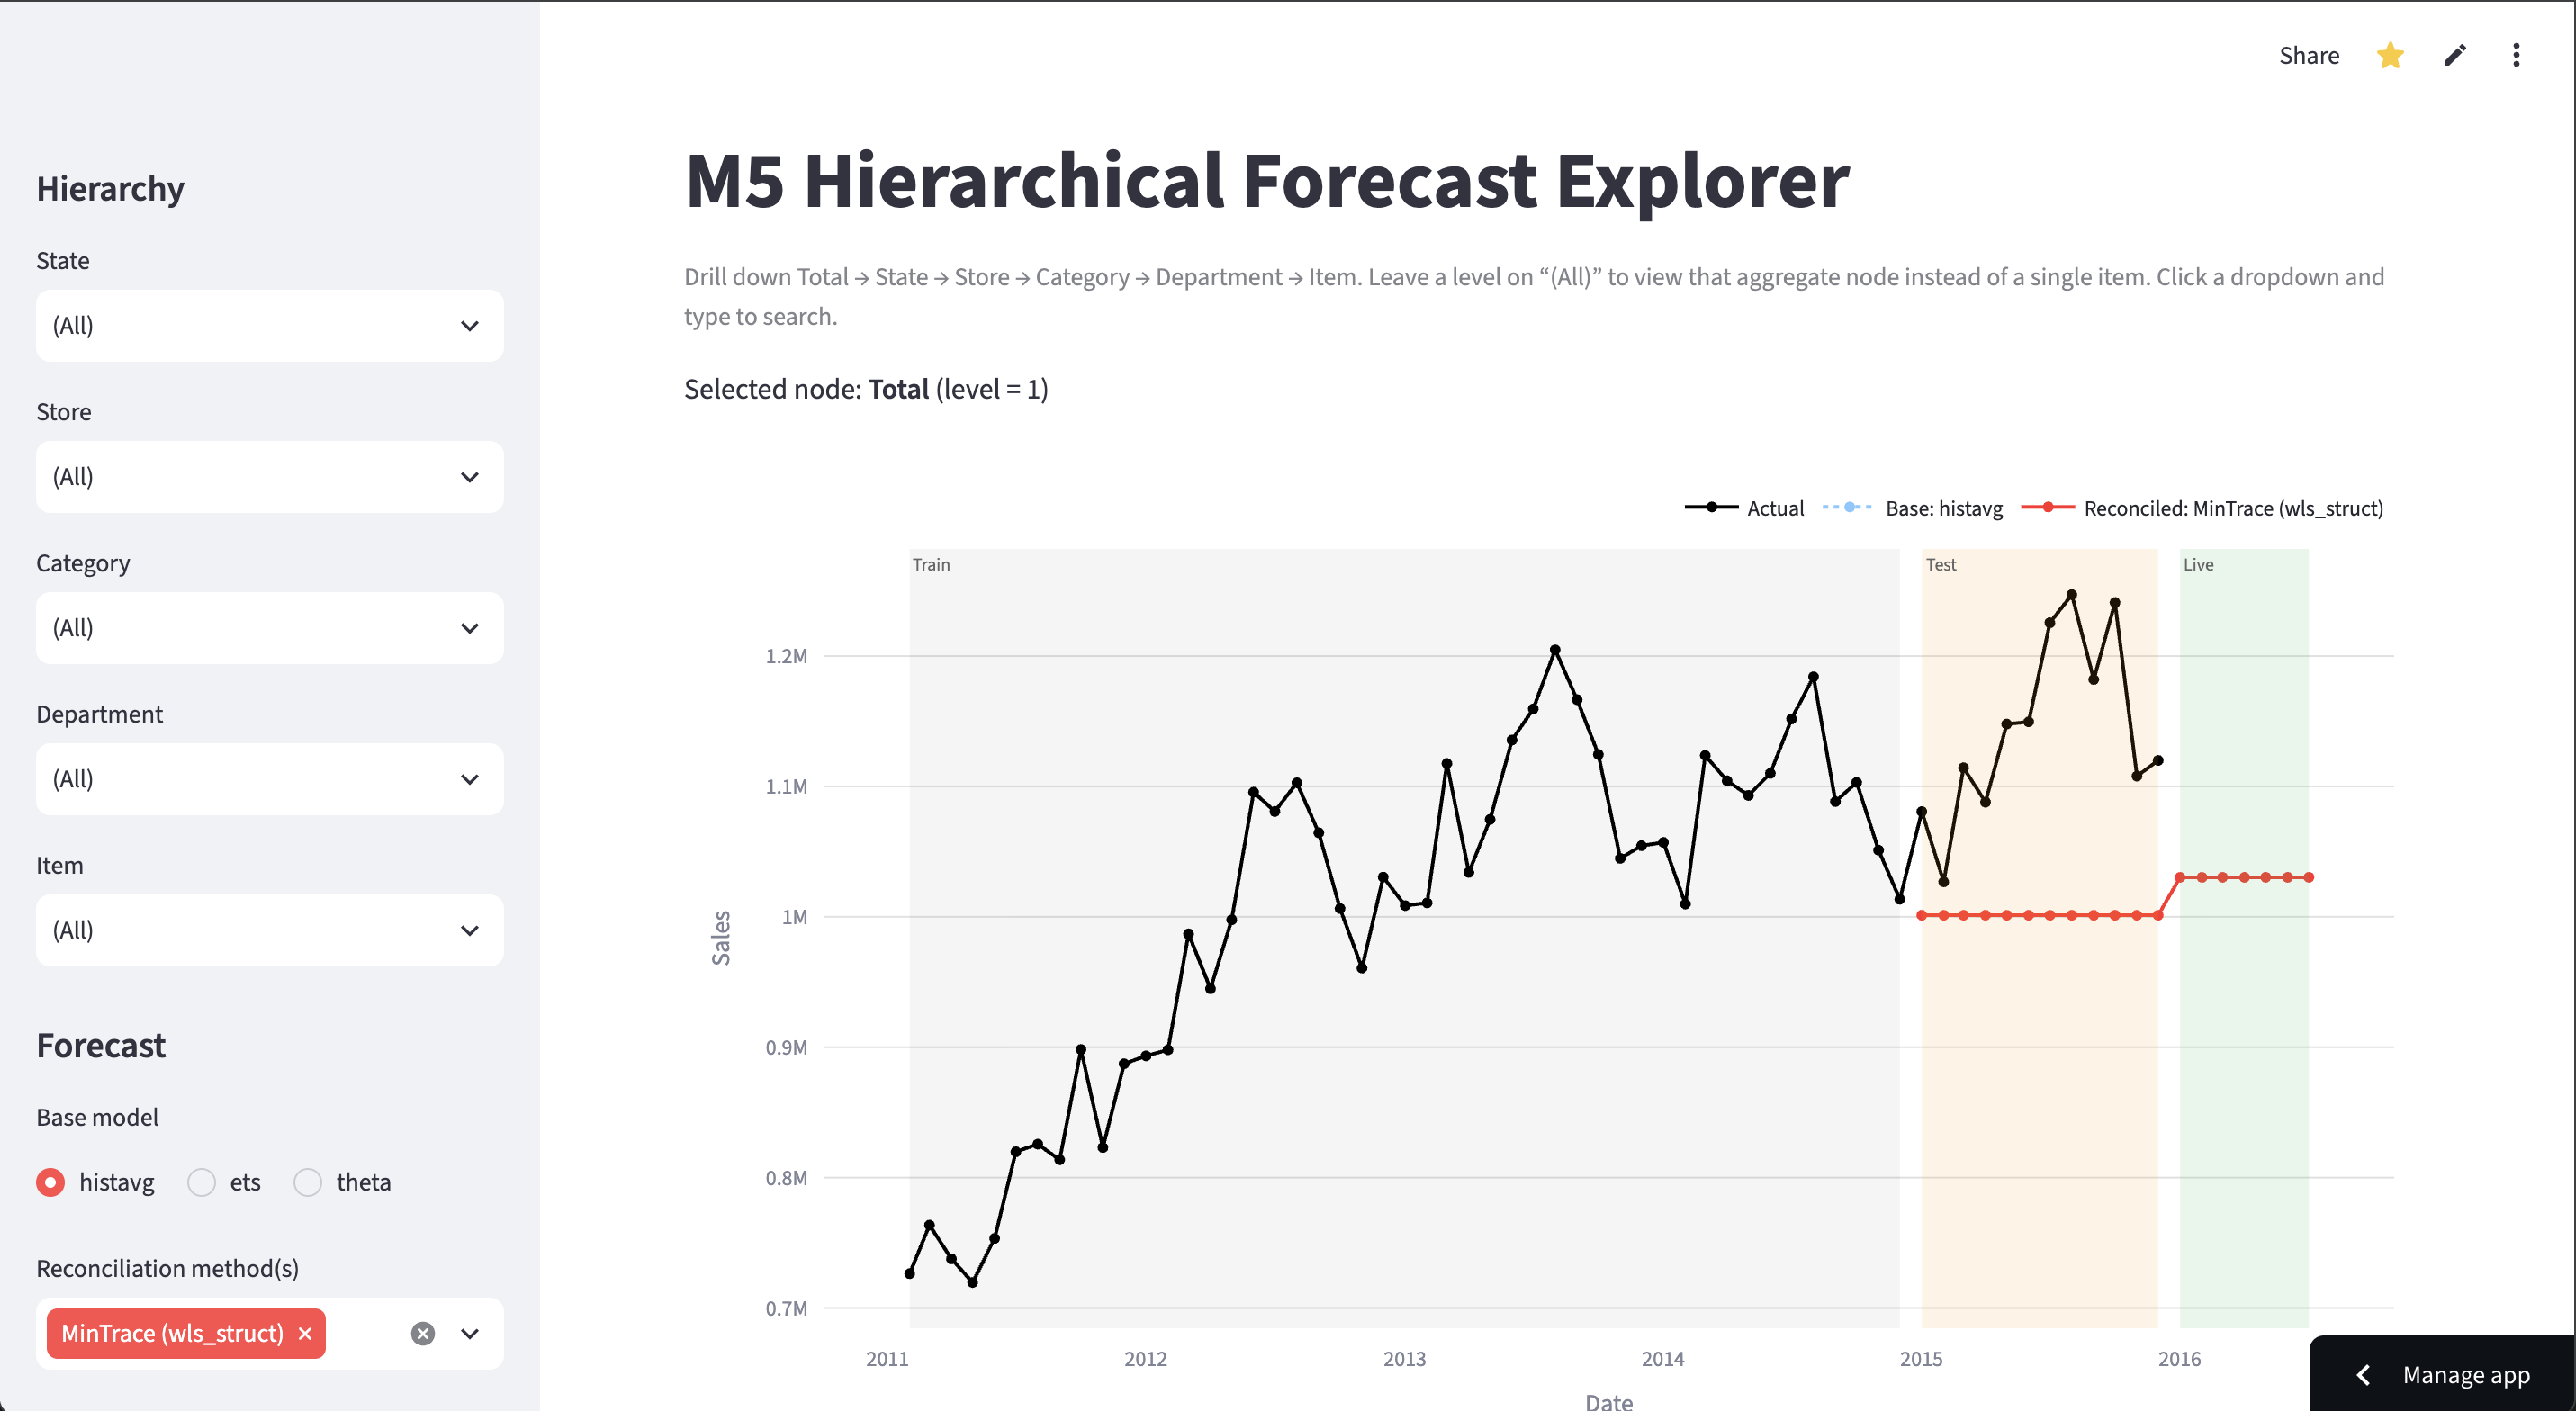
\includegraphics[width=0.49\linewidth]{Images/08ApplicationDeployment/dashboardChartLightMode}
	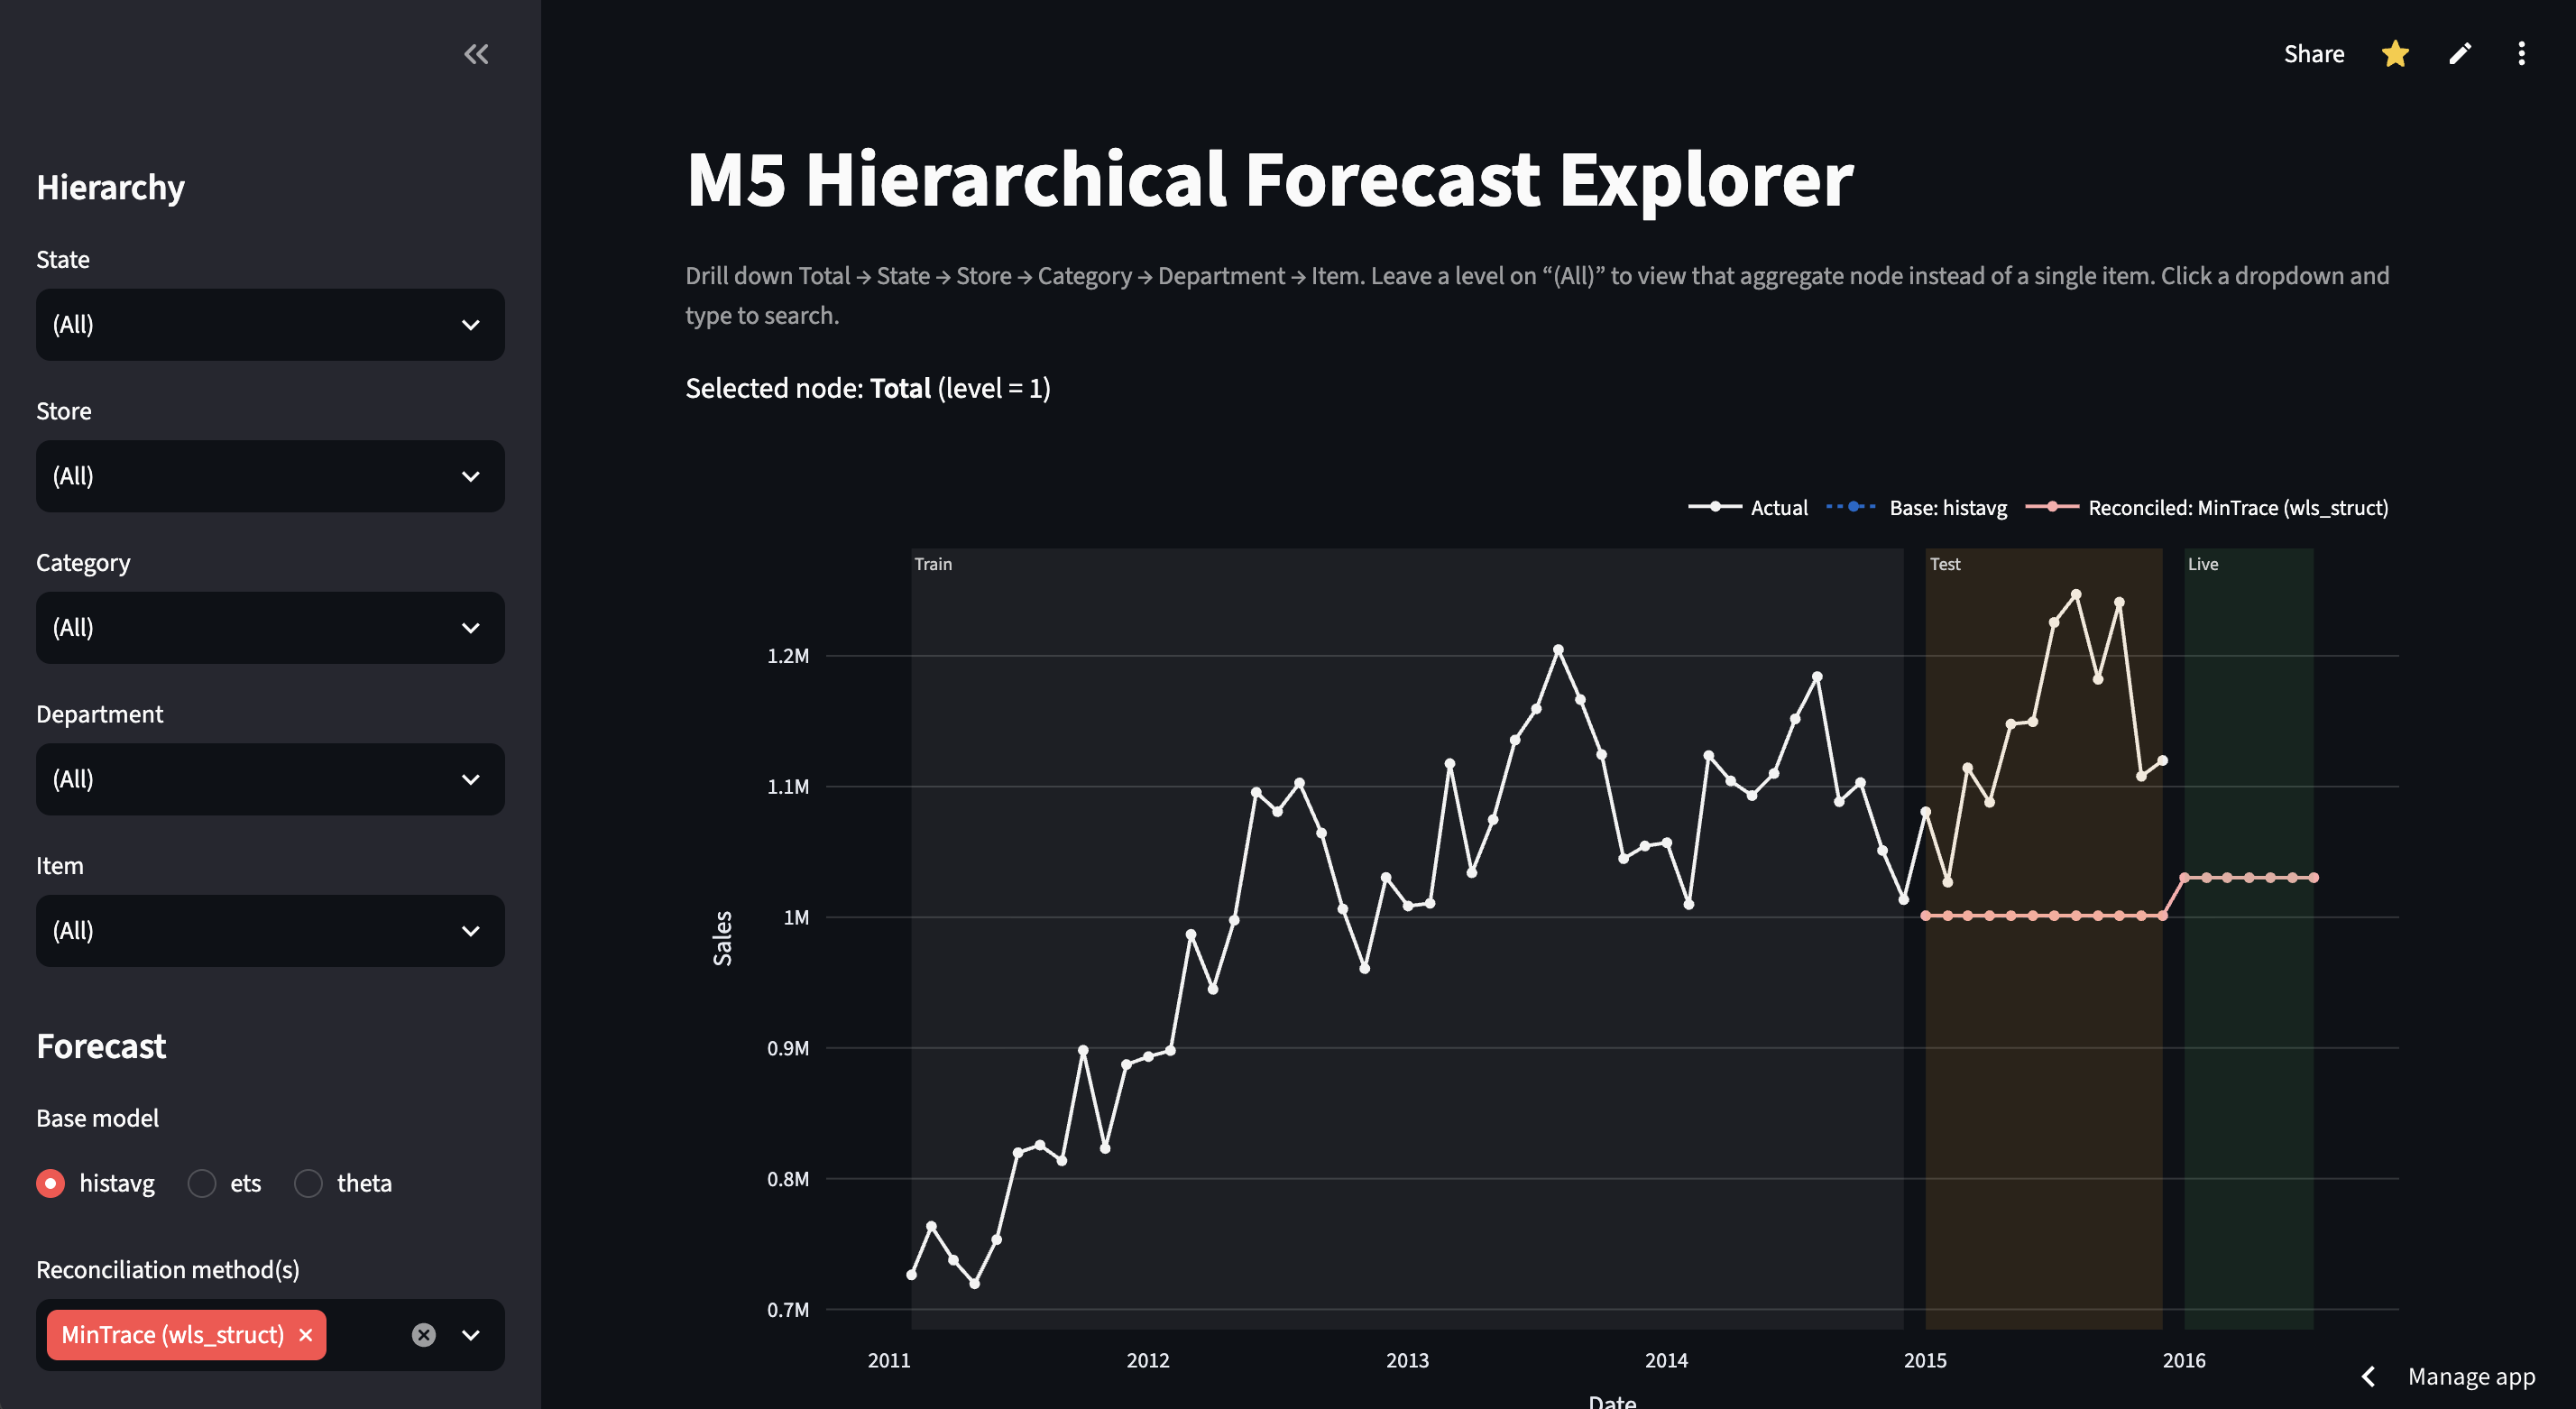
\includegraphics[width=0.49\linewidth]{Images/08ApplicationDeployment/dashboardChartDarkMode}
	\caption{The forecast chart in light mode (left) and dark mode (right), showing the shaded train/test/live regions.}\label{fig:dashboardChart}
\end{figure}

\section{Theme Sensing}
\label{sec:themeSensing}

Rather than adding a separate light/dark toggle to the app's own interface, the dashboard reads Streamlit's actual active theme directly from the browser via the \texttt{st\_theme()} call \cite{StTheme:2026}. This package is distributed on PyPI as \texttt{st-theme} and imported as \texttt{streamlit\_theme} -- a naming mismatch worth stating explicitly, since \texttt{streamlit-theme} is in fact a separate, unrelated PyPI package for setting a custom theme rather than reading the active one; \texttt{app/requirements.txt} documents this distinction to prevent the wrong package being installed by name alone. \texttt{st\_theme()} itself reflects whatever the user has set at the platform level, including a "use system setting" choice. The result is cached in \texttt{st.session\_state} the first time it is available, and a single boolean derived from it decides which colour palette the chart in Section~\ref{sec:chartDesign} uses. This keeps the dashboard's own theme behaviour consistent with the rest of the user's Streamlit session, without asking them to set the same preference twice.

\section{Deployment on Streamlit Community Cloud}
\label{sec:streamlitDeployment}

Because Streamlit Community Cloud only ever executes \texttt{app/streamlit\_app.py} and never re-runs the notebooks, the four Parquet files described in Section~\ref{sec:dataContracts} have to already exist in the repository at deploy time; the app has no way to regenerate them itself. The app imports \texttt{config.py} by explicitly appending the repository root to \texttt{sys.path} before importing it, which is necessary because Community Cloud always sets the working directory to the repository root rather than to the \texttt{app/} folder the script itself lives in -- a relative import that works when run locally from \texttt{app/} would otherwise fail on the deployed service. The dependencies actually installed on Community Cloud come from \texttt{app/requirements.txt}, a separate, smaller manifest than the \texttt{requirements-pipeline.txt} used to run the notebooks locally (Chapter~\ref{chap:devToDeployment}), since the deployed app needs Streamlit, Plotly, and \texttt{st-theme} (Section~\ref{sec:themeSensing}) but none of the modelling libraries the pipeline depends on. The same script can also be run locally with \texttt{streamlit run app/streamlit\_app.py} against a local checkout of the same Parquet files, which is how the app is checked before every deploy.

\section{Deployment Flow}
\label{sec:deploymentFlow}

Figure~\ref{fig:deploymentFlow} traces the full path from a local pipeline run to a served dashboard. Running \texttt{02\_pipeline.ipynb} writes the four Parquet files into \texttt{Code/artifacts/dashboard\_data/}; committing and pushing that folder to GitHub is what makes updated forecasts available to the deployed app, since Community Cloud has no other way to see new data. A push to the connected repository triggers Community Cloud to rebuild the app, which then boots, loads the Parquet files through \texttt{config.py}'s paths exactly as a local run would, and serves the resulting dashboard to the browser. Because this whole chain is triggered by a Git push rather than a scheduled job, the dashboard reflects whatever was last pushed, not necessarily the most recently run pipeline -- re-running the pipeline without pushing the updated Parquet files leaves the deployed dashboard unchanged.

\begin{figure}[H]
	\centering
	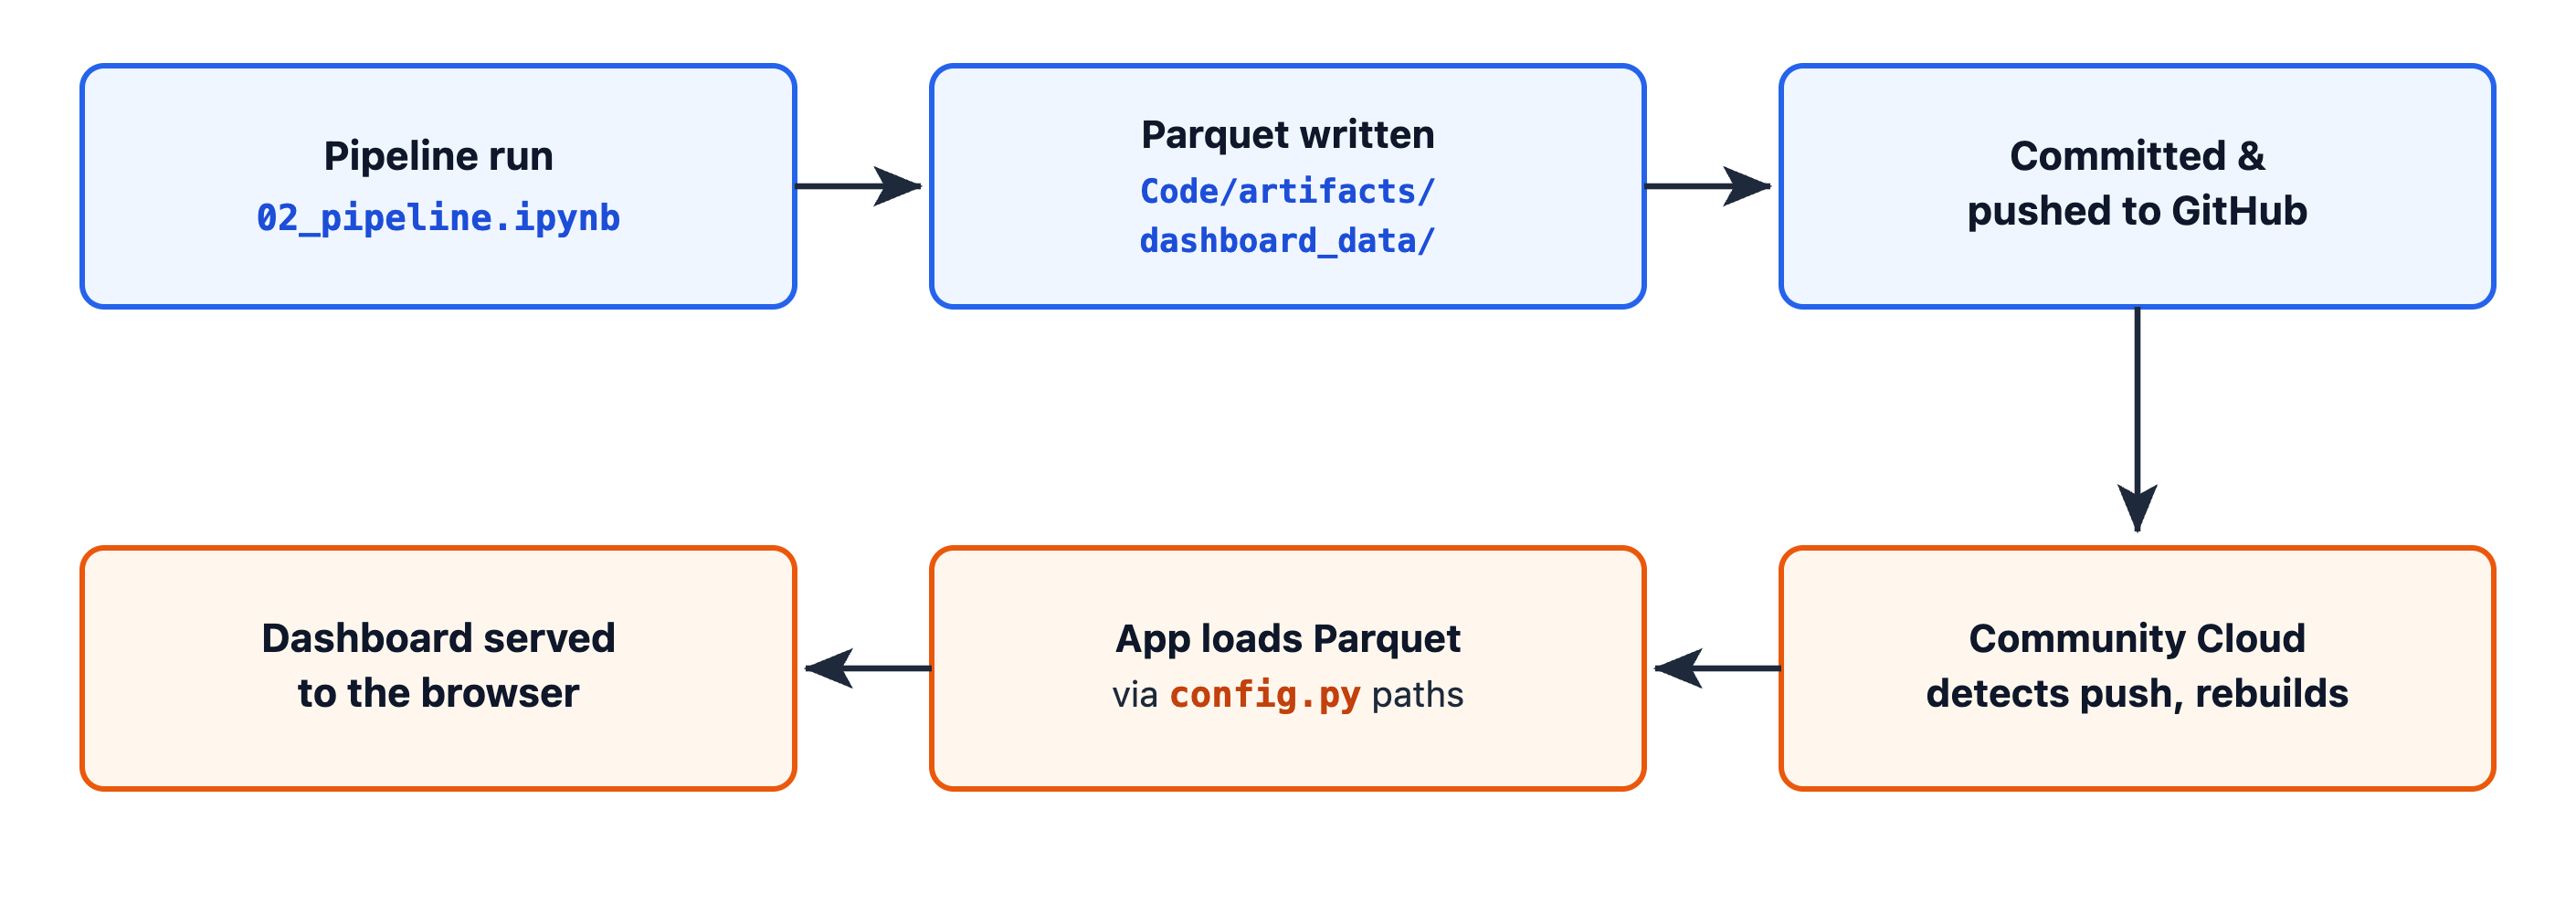
\includegraphics[width=1\linewidth]{Images/08ApplicationDeployment/deploymentFlowDiagram}
	\caption{The deployment flow from a local pipeline run to the served dashboard.}\label{fig:deploymentFlow}
\end{figure}


